\documentclass[12pt,journal]{IEEEtran} 
%\documentclass[draft,12pt]{article}  to suppress figs for fast compilation
%\documentclass[12pt, letter, twocolumn]{article}

\usepackage{amssymb,amsmath}
\usepackage{lmodern}
\usepackage{ifxetex,ifluatex}
\usepackage{fixltx2e} % provides \textsubscript
\usepackage[left=1in,right=1in,top=1in,bottom=1in]{geometry}
\usepackage{natbib}
\usepackage{xcolor}
\setcitestyle{authoryear,open={(},close={)}}
\usepackage{soul}
\usepackage{fancyhdr}
\usepackage{enumitem}
\usepackage{multirow}
\usepackage{multicol}
\usepackage{pdfpages} %https://tex.stackexchange.com/questions/21248/how-to-add-a-page-number-to-the-included-pdf-pages
\usepackage{float}
\usepackage{forest,array}
%\usepackage{csvsimple}
\usepackage{textcomp}
\usetikzlibrary{shadows}
\newcolumntype{C}[2]{>{\centering}p{#1}}
%\usepackage[font=footnotesize,labelfont=bf]{caption}
\usepackage{wrapfig,lipsum,booktabs}
\usepackage{wrapfig}
\usepackage{pdflscape}

%\usepackage{hyperref}

\usepackage{array}
\newcolumntype{L}[1]{>{\raggedright\let\newline\\\arraybackslash\hspace{0pt}}m{#1}}
\newcolumntype{C}[1]{>{\centering\let\newline\\\arraybackslash\hspace{0pt}}m{#1}}
\newcolumntype{R}[1]{>{\raggedleft\let\newline\\\arraybackslash\hspace{0pt}}m{#1}}

\pagestyle{fancy}
%this toggle commands turns on and off PDFs that you want to include such as budget, letters of support, CVs, etc...
\newtoggle{subPDFs} 
\toggletrue{subPDFs} %for compiling on overleaf
%\renewcommand{\thesection}{\@arabic\c@section}


\renewcommand{\thesection}{\Alph{section}.}

%ADD MISSION NAME HERE:
\newcommand{\headertext}{My Mission- NNH17ZDA004O-APEXMO }
\newcommand{\institution}{A University\ }

\lhead{\headertext\hfill \thesection} % page numbers and title on every page so reviewers don't get lost!
\cfoot{\thepage.\\  \tiny{Use or disclosure of the data on this page is subject to the restrictions on the title page of this proposal}}

% use upquote if available, for straight quotes in verbatim environments
\IfFileExists{upquote.sty}{\usepackage{upquote}}{}
% use microtype if available
%\IfFileExists{microtype.sty}{%
%\usepackage[]{microtype}
%\UseMicrotypeSet[protrusion]{basicmath} % disable protrusion for tt fonts
%}{}
\PassOptionsToPackage{hyphens}{url} % url is loaded by hyperref
\usepackage[unicode=true]{hyperref}
\hypersetup{
            pdfborder={0 0 0},
            breaklinks=true}
\urlstyle{same}  % don't use monospace font for urls
\usepackage{longtable,booktabs}
% Fix footnotes in tables (requires footnote package)
\IfFileExists{footnote.sty}{\usepackage{footnote}\makesavenoteenv{long table}}{}
\usepackage{graphicx,grffile} %set [draft] saves compile time{
\usepackage{subcaption}
\usepackage{glossaries}
\makeglossaries
\makeatletter
\def\maxwidth{\ifdim\Gin@nat@width>\linewidth\linewidth\else\Gin@nat@width\fi}
\def\maxheight{\ifdim\Gin@nat@height>\textheight\textheight\else\Gin@nat@height\fi}
\makeatother
% Scale images if necessary, so that they will not overflow the page
% margins by default, and it is still possible to overwrite the defaults
% using explicit options in \includegraphics[width, height, ...]{}
\setkeys{Gin}{width=\maxwidth,height=\maxheight,keepaspectratio}
\IfFileExists{parskip.sty}{%
\usepackage{parskip}
}{% else
\setlength{\parindent}{0pt}
\setlength{\parskip}{3pt plus 2pt minus 1pt}
}
\setlength{\emergencystretch}{3em}  % prevent overfull lines
\providecommand{\tightlist}{%
  \setlength{\itemsep}{0pt}\setlength{\parskip}{0pt}}
\setcounter{secnumdepth}{0}  %https://tex.stackexchange.com/questions/11668/adding-unnumbered-sections-to-toc
% Redefines (sub)paragraphs to behave more like sections 


% create "fakesections" that don't have text but show up in TOC:
%https://tex.stackexchange.com/questions/443701/how-to-remove-the-section-title-and-the-section-counter?noredirect=1&lq=1
\newcommand{\fakesection}[1]{%
  \par\refstepcounter{section}% Increase section counter
  %\sectionmark{#1}% Add section mark (header)
  \addcontentsline{toc}{section}{ #1}% Add section to ToC
  % Add more content here, if needed.
}
\newcommand{\fakesubsection}[1]{%
  %\par\refstepcounter{section}% Increase section counter
  %\sectionmark{#1}% Add section mark (header)
  \addcontentsline{toc}{subsection}{ #1}% Add section to ToC
  % Add more content here, if needed.
}


\renewcommand*{\thefootnote}{\fnsymbol{footnote}}

\date{}

\begin{document}
\let\la=\lesssim            % For Springer A&A compliance... 
\let\ga=\gtrsim 
\newcommand\arcdeg{\mbox{$^\circ$}}% 
\newcommand\arcmin{\mbox{$^\prime$}}%  \citep
\newcommand\arcsec{\mbox{$^{\prime\prime}$}}% 
\newcommand\arcs{\mbox{$^{\prime\prime}$}}% 

\def\farcs{\hbox{$.\!\!^{\prime\prime}$}}


%custom commands:

%ewan's usual acronym list:https://gist.github.com/douglase/78b39cfa4501f0ce43fe
% astronomical and space physics acronyms for use with LaTeX glossaries package.

%to copy without git, try: 
% wget https://gist.githubusercontent.com/douglase/78b39cfa4501f0ce43fe/raw//acronyms.tex
% or if you want to overwrite:
% curl -O https://gist.githubusercontent.com/douglase/78b39cfa4501f0ce43fe/raw//acronyms.tex

%units
\newacronym{AU}{AU}{astronomical Unit [1.5e11 m]}  
\newacronym{pc}{pc}{parsec}
\newacronym{mas}{mas}{milliarcsecond}
\newacronym{nm}{nm}{nanometer}
\newacronym{CTE}{CTE}{coefficient of thermal expansion}

%objects
\newacronym{smc}{SMC}{Small Magellanic Cloud}
\newacronym{lmc}{LMC}{Large Magellanic Cloud}
\newacronym{ism}{ISM}{interstellar medium}
\newacronym{mw}{MW}{Milky Way}
\newacronym{epseri}{$\epsilon$ Eri}{Epsilon Eridani}
\newacronym{EKB}{EKB}{Edgeworth-Kuiper Belt}


%radiative transfer
\newacronym{CFR}{CFR}{Complete Frequency Redistribution}

%organizations
\newacronym{nasa}{NASA}{National Aeronautics and Space Agency}
\newacronym{esa}{ESA}{European Space Agency}
\newacronym{omi}{OMI}{\textit{Optical Mechanics Inc.}}
\newacronym{gsfc}{GSFC}{\gls{nasa} Goddard Space Flight Center}
\newacronym{stsci}{STScI}{Space Telescope Science Institute}
\newacronym{nsroc}{NSROC}{\gls{nasa} Sounding Rocket Operations Contract}
\newacronym{wff}{WFF}{\gls{nasa} Wallops Flight Facility}
\newacronym{wsmr}{WSMR}{White Sands Missile Range}

%technologies and sensors
\newacronym{irac}{IRAC}{Infrared Array Camera}
\newacronym[plural=CCDs, firstplural=charge-coupled devices (CCDs)]{ccd}{CCD}{charge-coupled device}
\newacronym[plural=EMCCDs, firstplural=electron multiplying charge-coupled devices (EMCCDs)]{EMCCD}{EMCCD}{electron multiplying charge-coupled device}

\newacronym{DM}{DM}{Deformable Mirror}
\newacronym{MCP}{MCP}{ Microchannel Plate }
\newacronym{ipc}{IPC}{Image Proportional Counter}
\newacronym{cots}{COTS}{Commercial Off-The-Shelf}
\newacronym{ISR}{ISR}{Incoherent Scatter Radar }
\newacronym{atcamera}{AT}{Angle Tracker}
\newacronym{MEMS}{MEMS}{microelectromechanical systems}
\newacronym{QE}{QE}{quantum efficiency}
\newacronym{RTD}{RTD}{Resistance Temperature Detector}
\newacronym{PID}{PID}{Proportional-Integral-Derivative}
\newacronym{PRNU}{PRNU}{photo response non-uniformity}
\newacronym{DSNU}{PRNU}{dark signal non-uniformity}
\newacronym{CMOS}{CMOS}{complementary metal–oxide–semiconductor}
\newacronym{TRL}{TRL}{technology readiness level}

%optics
\newacronym{FOV}{FOV}{field-of-view}
\newacronym{NIR}{NIR}{near-infrared}
\newacronym{PV}{PV}{Peak-to-Valley}
\newacronym{MRF}{MRF}{Magnetorheological finishing}
\newacronym{AO}{AO}{Adaptive Optics}
\newacronym{TTP}{TTP}{tip, tilt, and piston}
\newacronym{FPS}{FPS}{fine pointing system}
\newacronym{SHWFS}{SHWFS}{Shack-Hartmann Wavefront Sensor}
\newacronym{OAP}{OAP}{off-axis parabola}
\newacronym{LGS}{LGS}{laser guide star}
\newacronym{WFCS}{WFCS}{wavefront control system}
\newacronym{OPD}{OPD}{optical path difference}

%%sounding Rockets:
\newacronym{acs}{ACS}{Attitude Control System}
\newacronym{orsa}{ORSA}{Ogive Recovery System Assembly}
\newacronym{gse}{GSE}{Ground Station Equipment}
\newacronym{FSM}{FSM}{Fast Steering Mirror}


%%high contrast imaging:
\newacronym{WFS}{WFS}{wavefront sensor}
\newacronym{LSI}{LSI}{Lateral Shearing Interferometer}
\newacronym{VVC}{VVC}{Vector Vortex Coronagraph}
\newacronym{VNC}{VNC}{Visible Nulling Coronagraph}
\newacronym{CGI}{CGI}{Coronagraph Instrument}
\newacronym{IWA}{IWA}{Inner Working Angle}
\newacronym{OWA}{OWA}{Outer Working Angle}
\newacronym{NPZT}{N-PZT}{Nuller piezoelectric transducer}
\newacronym{ZWFS}{ZWFS}{Zernike wavefront sensor}
\newacronym{SPC}{SPC}{Shaped Pupil Coronagraph}
\newacronym{HLC}{HLC}{Hybrid-Lyot Coronagraph}
\newacronym{ADI}{ADI}{angular differential imaging}
\newacronym{RDI}{RDI}{reference differential imaging}

%observatories and instruments
\newacronym{HST}{HST}{Hubble Space Telescope}
\newacronym{GPS}{GPS}{Global Positioning System}
\newacronym{ISS}{ISS}{International Space Station}
\newacronym[description=Advanced CCD Imaging Spectrometer]{acis}{ACIS}{Advanced \gls{ccd} Imaging Spectrometer}
\newacronym{stis}{STIS}{\textit{Space Telescope Imaging Spectrograph}}
\newacronym{mcp}{MCP}{Microchannel Plate}
\newacronym{jwst}{JWST}{$\textit{James Webb Space Telescope}$}
\newacronym{fuse}{FUSE}{$\textit{FUSE}$}
\newacronym{galex}{GALEX}{$\textit{Galaxy Evolution Explorer}$}
\newacronym{spitzer}{Spitzer}{$\textit{Spitzer Space Telescope}$}
\newacronym{mips}{MIPS}{Multiband Imaging Photometer for \gls{spitzer}}
\newacronym{gissmo}{GISSMO}{Gas Ionization Solar Spectral Monitor}
\newacronym{iue}{IUE}{International Ultraviolet Explorer}
\newacronym{spinr}{SPINR}{$\textit{Spectrograph for Photometric Imaging with Numeric Reconstruction}$}
\newacronym{imager}{IMAGER}{$\textit{Interstellar Medium Absorption Gradient Experiment Rocket}$}
\newacronym{TPF-C}{TPF-C}{Terrestrial Planet Finder Coronagraph}
\newacronym{RAIDS}{RAIDS}{Atmospheric and Ionospheric Detection System }
\newacronym{mama}{MAMA}{Multi-Anode Microchannel Array}
\newacronym{ATLAST}{ATLAST}{Advanced Technology Large Aperture Space Telescope}
\newacronym{PICTURE}{PICTURE}{Planet Imaging Concept Testbed Using a Rocket Experiment}
\newacronym{LITES}{LITES}{Limb-imaging Ionospheric and Thermospheric
Extreme-ultraviolet Spectrograph}
\newacronym{LBT}{LBT}{Large Binocular Telescope}
\newacronym{LBTI}{LBTI}{Large Binocular Telescope Interferometer}
\newacronym{KIN}{KIN}{Keck Interferometer Nuller}
\newacronym{SHARPI}{SHARPI}{Solar High-Angular Resolution Photometric Imager}
\newacronym{IRAS}{IRAS}{Infrared Astronomical Satellite}
\newacronym{HARPS}{HARPS}{High Accuracy Radial velocity Planetary}
\newacronym{hstSTIS}{STIS}{Space Telescope Imaging Spectrograph}
\newacronym{spitzerIRAC}{IRAC}{Infrared Array Camera}
\newacronym{spitzerMIPS}{MIPS}{Multiband Imaging Photometer for Spitzer}
\newacronym{spitzerIRS}{IRS}{Infrared Spectrograph}
\newacronym{CHARA}{CHARA}{Center for High Angular Resolution Astronomy}
\newacronym{wfirst-afta}{WFIRST-AFTA}{Wide-Field InfrarRed Survey
Telescope-Astrophysics Focused Telescope Assets}
\newacronym{GPI}{GPI}{Gemini Planet Imager}
\newacronym{WFIRST}{WFIRST}{Wide-Field InfrarRed Survey Telescope}
\newacronym{HabEx}{HabEx}{Habitable Exoplanet Observatory Mission Concept}
\newacronym{LUVOIR}{LUVOIR}{Large UV/Optical/Infrared Surveyor}
\newacronym{FGS}{FGS}{Fine Guidance Sensor}
\newacronym{STIS}{STIS}{Space Telescope Imaging Spectrograph}
\newacronym{MGHPCC}{MGHPCC}{Massachusetts Green High Performance
Computing Center}
\newacronym{WISE}{WISE}{Wide-field Infrared Survey Explorer}
\newacronym{ALMA}{ALMA}{Atacama Large Millimeter Array}
\newacronym{GRAIL}{GRAIL}{Gravity Recovery and Interior Laboratory}

%software
\newacronym{AURIC}{AURIC}{The Atmospheric Ultraviolet Radiance Integrated Code} 
\newacronym{FFT}{FFT}{Fast Fourier Transform  }
\newacronym{MODTRAN}{MODTRAN   }{ MODerate resolution atmospheric TRANsmission }
\newacronym{idl}{IDL}{$\textit {Interactive Data Language}$}
\newacronym[sort=NED,description=NASA/IPAC Extragalactic Database]{ned}{NED}{\gls{nasa}/\gls{ipac} Extragalactic Database}
\newacronym{iraf}{IRAF}{Image Reduction and Analysis Facility}
\newacronym{wcs}{WCS}{World Coordinate System}
\newacronym{pegase}{PEGASE}{$\textit{Projet d'Etude des GAlaxies par Synthese Evolutive}$}
\newacronym{dirty}{DIRTY}{$\textit{DustI Radiative Transfer, Yeah!}$}
\newacronym{CUDA}{CUDA}{Compute Unified Device Architecture}
\newacronym{KLIP}{KLIP}{Karhunen-Lo`eve Image Processing}

%earth's atmosphere and ionosphere:
\newacronym{MSIS}{MSIS}{Mass Spectrometer Incoherent Scatter Radar}
\newacronym{nmf2}{$N_m$}{F2-Region Peak density}
\newacronym{hmf2}{$h_m$}{F2-Region Peak height}
\newacronym{H}{$H$}{F2-Region Scale Height}

%misc jargon
\newacronym{isr}{ISR}{Incoherent Scatter Radar}
\newacronym[description=TLA Within Another Acronym]{twaa}{TWAA}{\gls{tla} Within Another Acronym}
\newacronym[plural=SNe, firstplural=Supernovae (SNe)]{sn}{SN}{Supernova}
\newacronym{EUV}{EUV}{Extreme-Ultraviolet }
\newacronym{EUVS}{EUVS}{\gls{EUV} Spectrograph}
\newacronym{F2}{F2}{Ionospheric Chapman F Layer }
\newacronym{F10.7}{F10.7}{ 10.7 cm radio flux [10$^{-22}$ W m$^{-2}$ Hz$^{-1}$]  }
\newacronym{FUV}{FUV}{far-ultraviolet }
\newacronym{IR}{IR}{infrared}
\newacronym{MUV}{MUV}{mid-ultraviolet }
\newacronym{NUV}{NUV}{near-ultraviolet }
\newacronym{O$^+$}{O$^+$}{Singly Ionized Oxygen  Atom }
\newacronym{OI}{OI}{Neutral Atomic Oxygen Spectroscopic State }
\newacronym{OII}{OII}{Singly Ionized Atomic Oxygen Spectroscopic State }
\newacronym{PSF}{PSF}{point spread function}
\newacronym{$R_E$}{$R_E$}{Earth radii [$\approx$ 6400 km]  }
\newacronym{RV}{RV}{radial velocity}
\newacronym{UV}{UV}{ultraviolet }
\newacronym{WFE}{WFE}{wavefront error}
\newacronym{sed}{SED}{spectral energy distribution}
\newacronym{nir}{NIR}{near-infrared}
\newacronym{mir}{MIR}{mid-infrared}
\newacronym{ir}{IR}{infrared}
\newacronym{uv}{UV}{ultraviolet}
\newacronym[plural=PAHs, firstplural=Polycyclic Aromatic Hydrocarbons (PAHs)]{pah}{PAH}{Polycyclic Aromatic Hydrocarbon}
\newacronym{obsid}{OBSID}{Observation Identification}
\newacronym{SZA}{SZA}{Solar Zenith Angle}
\newacronym{TLE}{TLE}{Two Line Element set}
\newacronym{DOF}{DOF}{degrees-of-freedom}
\newacronym{PZT}{PZT}{lead zirconate titanate}
\newacronym{ADCS}{ADCS}{attitude determination and control system}
\newacronym{COTS}{COTS}{commercial off-the-shelf}
\newacronym{CDH}{C$\&$DH}{command and data handling}
\newacronym{EPS}{EPS}{electrical power system}

%stats
\newacronym{PCA}{PCA}{principal component analysis}
\newacronym{fwhm}{FWHM}{full-width-half maximum}
\newacronym{RMS}{RMS}{root mean squared}
\newacronym{RMSE}{RMSE}{root mean squared error}
\newacronym{MCMC}{MCMC}{Marcov chain Monte Carlo}
\newacronym{DIT}{DIT}{discrete inverse theory}
\newacronym{SNR}{SNR}{signal-to-noise ratio}
\newacronym{PSD}{PSD}{power spectral density}
\newacronym{NMF}{NMF}{non-negative matrix factorization}

%custom acronyms


\pagenumbering{gobble}

 
\begin{titlepage}
\fakesection{A Cover Page}\label{sec:A}

% \includepdf[pages=-,angle=0]{CoverPage}
\clearpage
\iftoggle{subPDFs}{

The Optimum Space Telescope - A Proposal

Year Day Month


RESTRICTION ON USE AND DISCLOSURE OF PROPOSAL AND QUOTATION INFORMATION (DATA): 
}. \
\end{titlepage}

\newpage
\onecolumn
INVESTIGATION SUMMARY INFORMATION

Investigation Title: 

Proposing Organization: 

STATEMENT OF COMMITMENT: The \institution  is fully committed to the cost, schedule, and scientific and technical performance reflected in this document.


Principal Investigator: 
Authorizing Official:  



\newpage

\fakesection{B -Fact Sheet}\label{sec:fact_sheet}

\begin{landscape}
%add 2 page landscape factsheets
%\includepdf[pages=1,angle=90]{factsheet.pdf}
\end{landscape}

%financial facts:

\newpage

%advance section counter for TOC but don't add to TOC
\par\refstepcounter{section}% Increase section counter

\tableofcontents
\newpage

\pagenumbering{arabic} % restart page numbering

\twocolumn
\setcounter{page}{1}


\section{D - Scientific Investigation}\label{sec:D}
% (\textless{}=2pages)}{~}}{Objectives and Significance. (\textless{}=2 pages)~}}\label{h.dprclba34bww}
\par\refstepcounter{section}% Increase section counter, 
%Requirement B-15.This section shall describe the goals and objectives of the investigation, the compelling nature of the investigation, the investigation?s value to advancing the NASA?s objectives, and the relationship of the proposed investigation to past, current, and future investigations and missions. 
%\begin{multicols}{2} %uncomment for 2 column



\subsection{D.1 Introduction}
This proposal template uses demonstrates the use of acronyms that are automatically compiled in to a glossary, like \gls{HST}, \gls{UV}, and \gls{EMCCD}.

\subsection{D.2 Investigation Requirements and Baseline Investigation}
{Requirement B-16.This section shall describe the investigation to be performed, the types of measurements to be taken; the characteristics, precision, and accuracy required to attain the investigation objectives; and the projected instrument performance. This section shall describe the data to be returned in the course of the investigation. The quality (e.g., resolution, coverage, pointing accuracy, measurement precision, etc.) and quantity (bits, images, etc.) of data that must be returned shall be described. The relationship between the proposed data products (e.g., flight data, ancillary or calibration data, theoretical calculations, higher order analytical or data products, laboratory data, etc.) and the investigation objectives, as well as the expected results, shall be described. How the investigation products and data obtained will be used to fulfill the investigation requirements shall be demonstrated and supported by quantitative analysis. These descriptions shall constitute the Baseline Investigation. 

Requirement B-17.Traceability from investigation goals to measurement requirements to instrument requirements (functional and performance), and to top-level mission requirements shall be provided in tabular form and supported by narrative discussion. Projected instrument performance shall be compared to instrument performance requirements. Table B1 of this appendix provides an example of a tabular Science Traceability Matrix, with examples of matrix elements. This matrix provides the reference points and tools needed to track overall investigation requirements, provide systems engineers with fundamental requirements needed to design the mission, show clearly the effects of any descoping or losses of elements, and facilitate identification of any resulting degradation to the investigation. }



\subsection{Science Requirements and Traceability}\label{sec:scitraceability}

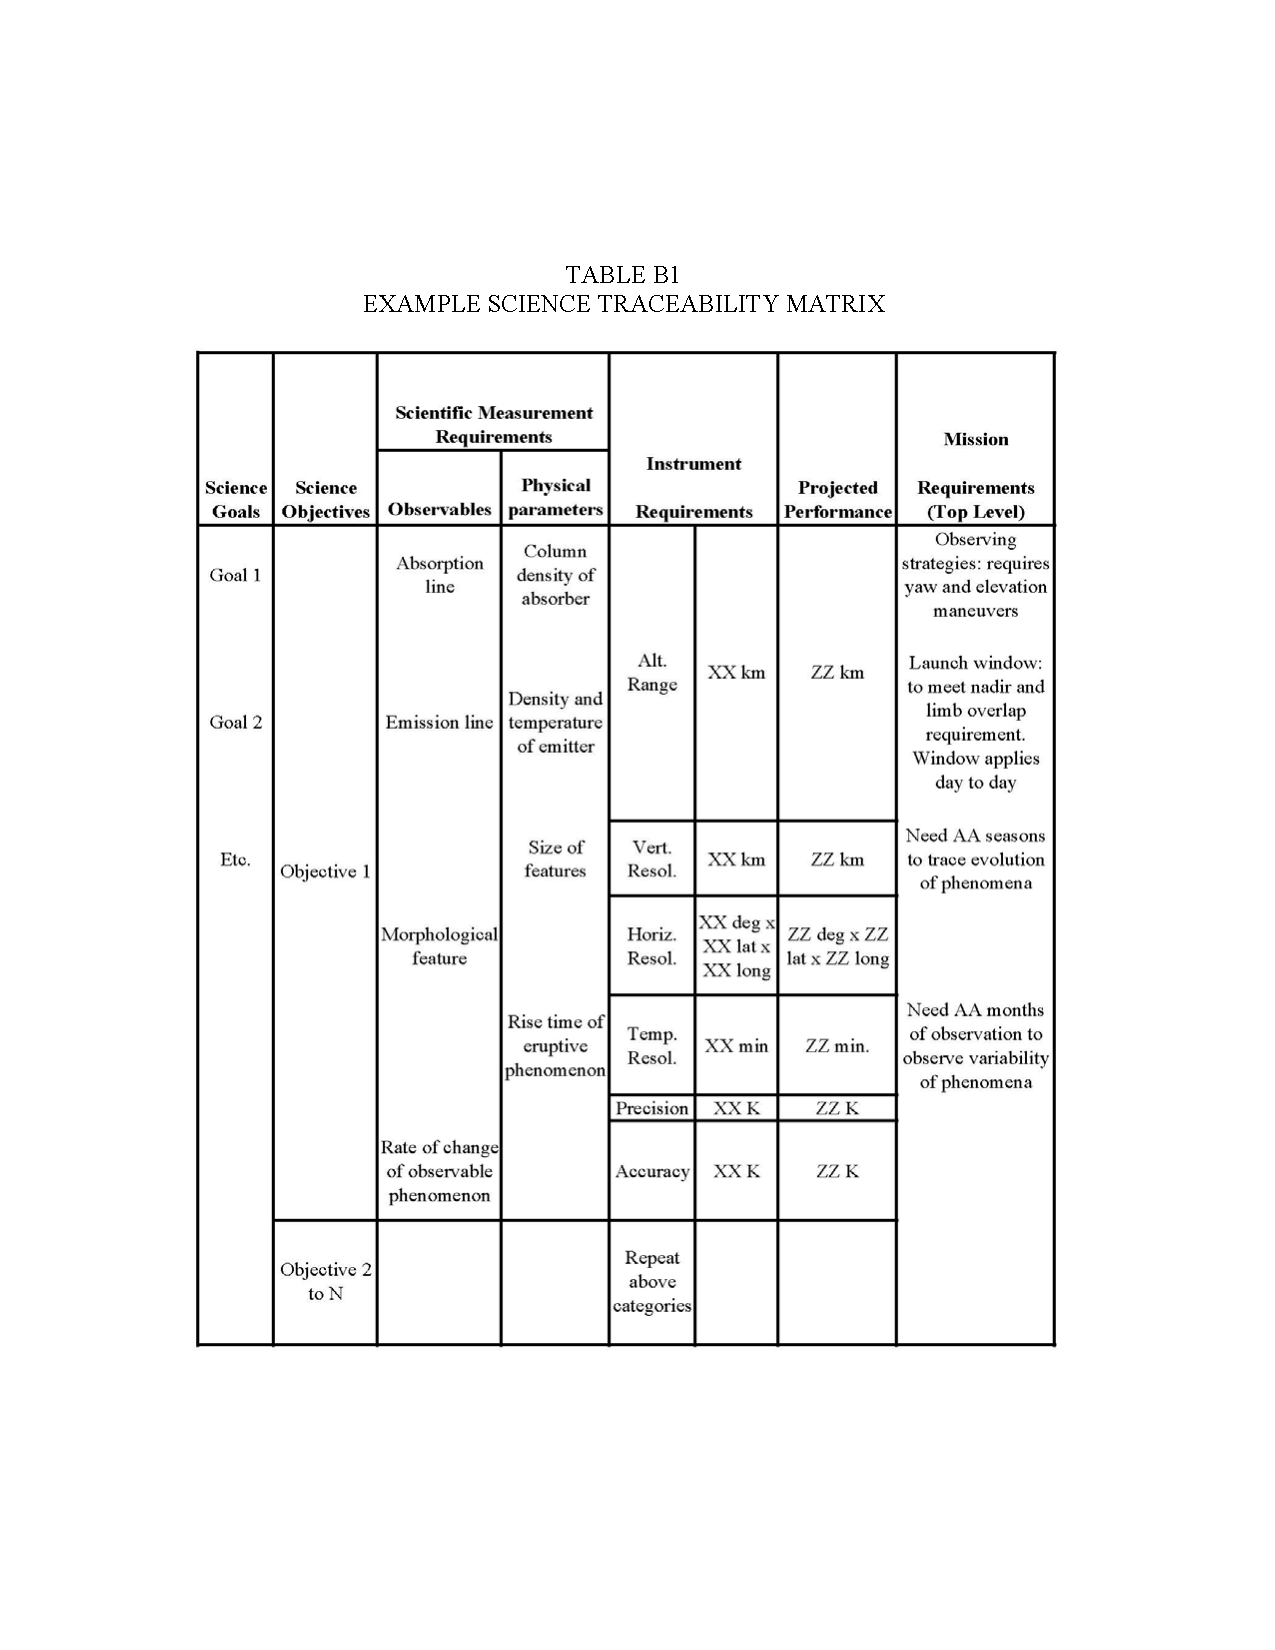
\includepdf[pages=-,pagecommand={},]{images/B1_MIssionTraceabilityMatrix.pdf}\label{tab:scitraceability}



\subsection{D.3 Threshold Investigation}
%B-7 Requirement B-18.This section shall identify the minimum acceptable data and return for the investigation (the Threshold Investigation), below that the investigation would not be worth pursuing. The Threshold Investigation is identified with the ?Threshold Science Requirements? in NPR 7120.5E. The scientific, exploration, or technology value of the Threshold Investigation shall be discussed. NASA recognizes that, in some circumstances, the Threshold Investigation may be identical to the Baseline Investigation. In such cases, the proposer shall explain why there is no viable investigation below the Baseline Investigation

%\newpage
\section{E	Science Implementation, including optional SEO}%{<=5}{~pages)}
\par\refstepcounter{section}% Increase section counter

\subsection{E.1	Instrumentation}

%Requirement B-19.This section shall describe the instrumentation and the rationale for its selection. It shall identify the individual instruments and instrument systems, instrument subsystems, instrument components, and sample collection and preservation systems as applicable, including their characteristics and requirements, and indicate items that are proposed for development, as well as any existing instrumentation or design/flight heritage. It shall provide a clear understanding of how the concept will provide the required data, show how it can be accommodated by the spacecraft, demonstrate that instruments have the necessary unobstructed fields-of-view over the measurement period required, describe the technology readiness levels and the approach to bring each instrument to Technology Readiness Level (TRL) 6  ( or TRL 5 as applicable for NASA STMD calls) by Preliminary Design Review (PDR ). If no development plan is needed, the reasons for this shall be explicitly stated and the rationale shall be described. A preliminary description of each instrument design, with a block diagram showing the instrument subsystems and components, and their interfaces, along with a description of the estimated performance of the instrument, shall be included. These performance characteristics (that shall be considered as requirements on the flight system) shall include mass, power, volume, data rate(s), thermal, pointing (such as control, stability, jitter, drift, accuracy, etc.), spatial and spectral resolution, observable precision, retrieved parameter sensitivity and accuracy, and calibration requirements. This section shall demonstrate that the instrumentation can meet the measurement requirements, including factors such as retrieval results for each remote sensor, error analysis of the information in all sensors, vertical and horizontal resolution, signal-to-noise (S/N) calculations, etc. It shall also discuss environmental effects, such as radiation, temperature, and contamination, on each instrument?s measurement capabilities as a function of mission time.

%\begin{wraptable}{l}{8.5cm}\
\subsection{E.3	Science Mission Profile}
%Requirement B-22.This section shall discuss the observing profile, including all mission-relevant parameters, such as orbit, navigation accuracy, operational time lines (including observing periods, data transmission periods and techniques, and time-critical events), etc. The manner in that the proposed investigation objectives, selected instruments, and measurement requirements drive the proposed mission design and operations plan shall be  included in this discussion.

\subsubsection{Mission Requirements}\label{sec:sci_mission_req}

\subsubsection{Sky availability}

\subsubsection{Radiation}\label{sec:radiation_flux_rates}

\subsection{E.4	Data Plans}
%Requirement B-23.A schedule-based end-to-end data management plan, including approaches for data retrieval, validation, preliminary analysis, and archiving shall be described. The investigation products (e.g.,    flight data, ancillary or calibration data, theoretical calculations, higher order analytical or data products, laboratory data, etc.) shall be identified, including a list of the specific data products and the individual team members responsible for the data products. The plan shall identify the appropriate NASA data archive(s) and the formats and standards to be used.  It shall include an estimate of the raw data volume and a schedule for the submission to the data archive of raw and reduced data in physical units accessible to the science community.The data plan shall be in compliance with terms and conditions stated in the NASA Plan: Increasing Access to the Results of Scientific Research or a justification shall be included that this is not necessary given the nature of the work proposed. The data management plan (DMP) (see Section 4.4.1) shall be addressed as part of the Data Plan.

\subsection{E.5	Science Team}
%Requirement B-24.This section shall identify each member of the investigation team and his/her role and responsibilities. Resumes or curriculum vitae of investigation team members shall be included as appendices to the proposal (see Section J.3 of this appendix). The role of the PI and   each Co-investigator (Co-I) shall be explicitly defined, the necessity of that role shall be justified, and the funding source (NASA or contributor) shall be noted; the role of each collaborator shall be described and the funding source shall be noted. 


\subsection{E.6	Plan for Science Enhancement Option (SEO)} %2 page limit
%Requirement B-25.If a   Science-Exploration-Technology Enhancement Option (SEO ) is proposed, this section shall define and describe the proposed activities (see Section 5.2.5 of the AO


\clearpage
\section{F. Investigation Implementation}
\par\refstepcounter{section}% Increase section counter

\subsection{F.1 General Requirements and Mission Traceability}
%Requirement B-35.This section shall provide a description of the spaceflight mission that is proposed to enable the science investigation.In some areas (e.g.,instruments), the data requested may have already been presented in another section of the proposal (e.g., the Experiment Implementation section). In such a case, a proposal may provide a reference to that section and need not repeat the data in this section.

%Requirement B-36.The mission requirements that the investigation goals and objectives impose on the mission design elements, including mission design, instrument accommodation, spacecraft design, required launch vehicle capability, ground systems, communications approach, and mission operations plan, shall be provided in tabular form and supported by narrative discussion. Table B2 provides an example of a tabular Mission Traceability Matrix, with examples of matrix elements. Specific information that describes how the investigation imposes unique requirements on these mission design elements shall be included. This matrix, along with Table B1, provides the reference points and tools needed to track overall   mission requirements, provides systems engineers with fundamental requirements needed to design the mission, shows clearly the effects of any descoping or losses of mission elements, and facilitates identification of any resulting degradation to the investigation.
An overview of the payload requirements on the mission is given in Sec. \ref{sec:sci_mission_req} and the overall mission requirements are summarized in Table B. 

\subsection{Orbit and Concept of Operations}

\subsection{Spacecraft and Bus}

% Requirement B-37.NASA recognizes that the full depth of information requested in Requirement B-38 through Requirement B-49 may not be available for some aspects of mission implementation at this stage of mission design. In such cases, this section shall (i) describe the current design concept, (ii) explain why the design information is not complete, (iii) provide a time-based plan for completing the design, (iv) justify that the development of that aspect of the design is not required at this stage and that it is acceptable to develop details later, and (v) Explain why the lack of information at this stage does not translate into a risk to the proposer's ability to implement the mission as proposed. The approach for developing the required depth of information, along with a corresponding development schedule, shall be included among the plans for future activity. In cases where a mission is proposed at or near the PEA-specific Cost Cap, but depth of technical implementation detail is deferred, the proposal shall justify theadequacy of the proposed cost reserves to prevent increases beyond the PEA-specific Cost Cap during formulation and implementation of the mission.This requirement is levied to establish NASA?s standard for completeness of information necessary to support a comprehensive assessment of implementation feasibility and risk. The quality of the proposal?s response to this requirement contributes significantly to the quality of the TMC assessment. However, NASA recognizes the preliminary nature of Pre-Phase A proposals, and thus Requirement B-37   will apply to all cases where the required information cannot, for whatever reason, be provided.


\subsection{F.2 Mission Concept Descriptions }\label{sec:f2_concept}
%Requirement B-38.Designs for all elements of the mission shall be described in sufficient detail to demonstrate that the proposed concept meets all of the basic requirements for a space flightmission, including mission design, spacecraft design, and supporting ground systems. Discussion of how the various mission elements meet the Mission Functional Requirements shall be included. At a minimum, the following mission elements shall be addressed: mission design, flight system capabilities, mission operations, and any additional elements.
%Requirement B-39.Mission Design: This section shall address the following elements of mission design to the extent that they are applicable to the proposed mission and that they are known at the time of proposal submission. Any additional elements that are applicable to explaining the mission and demonstrating its feasibility shall also be addressed.
%?Launch readiness date;
%?Launch date flexibility; 
%?Mission duration; 
%?Orbit type (Earth orbit, heliocentric, etc.) and orbit information (semimajor axis, eccentricity,inclination, node time of day, argument of perigee, altitude, allowable dispersions), and/or trajectory design, as applicable to the proposed investigation; 
 

\subsubsection{Mission Duration}

\subsection{Flight System Capabilities:} 
%Requirement B-41.Flight System Capabilities: This section shall address the following flight system capabilities to the extent that they are applicable to the proposed mission and that they areknown at the time of proposal submission. Any additional elements that are applicable to expl   aining the mission and demonstrating its feasibility shall also be addressed.i.Spacecraft Parameters:a.Figure of the complete spacecraft/instrument system, on the launch vehicle andinflight, with major components labeled and approximate overall dimensions. b.Block diagram of the spacecraft subsystems and their components. ii.Subsystem descriptions including structure, telecommunications, thermal, power, propulsion (if required), attitude determination and control, command and data handling, in-flight fault management, flight software, and ground software. (Note that the discussion of the telecommunications subsystem should be limited to specifications, design, and proposed component hardware ? discussion of the link performance is addressed as part of the mission operations approach). Subsystem detail shall include to the extent possible the following information: (a)Propulsion, including (i) Delta-V budget; (ii) for each propulsion mode propulsion type(s) (monoprop, bi-prop, dual-mode, solar electric, etc.), engines and thrust levels, and specific impulse; (iii) propellant allocation (impulse vs. attitude control system); and (iv)propellant margin, including nominal (to meet Delta-V requirement) and additional (to meet mass growth).(b)Command and Data Handling, including (i) spacecraft housekeeping data rates fornominal and safing strategy; (ii) data storage unit size (Mbits); and (iii) maximum storagerecord and playbackf rate. (c)Power, including (i) expected power requirement for each mission phase; (ii) minimum power capability needed to meet all requirements; and (iii) associated battery Depth ofDischarge (DOD).(d)Attitude Determination and Control, including system pointing requirements and capabilities. Describe or define the following: (i) each spacecraft operational mode, including the sensors and actuators used, control method, and safing and/or contingency modes; (ii) attitude determination methodology and estimate of accuracy, including identifying whether ground post-processing is required to meet investigation needs; (iii) agility requirements for slews or scanning; (iv) appendage pointing requirements, including articulation control methods and deployment accommodations; (v) sensor selection and performance, including identifying mounting location and Field -Of-View (FOV); (vi) actuator selection and sizing, including identifying mounting location(s); (vii)  translational maneuver (Delta-V) control and accuracy; (viii) momentum management approach and mitigation of impacts on navigation accuracy, if applicable; (ix) on-orbit calibrations, if required, including expected accuracy; and (x) attitude control requirements for the spacecraft pointing control, pointing knowledge (at the instrument interface), pointing stability, or jitter.(e)Thermal control, including (i) temperature requirements including deltas, (ii) temperature control approach (i.e. passive vs. active), (iii) cooling loads, and (iv) special thermal design considerations (e.g., cryogenic instrument requirements).


%Requirement B-42.Additional Mission Elements:  This section shall address any other major mission elements (e.g., picosatellite dispenser, ESPA-ring  , etc.  ) to the extent that they are  applicable to the proposed mission and to the extent that they are known at the time of proposal submission. Any additional elements that are applicable to explaining the mission and demonstrating its feasibility shall also be discussed.i.Provide a block diagram and description of relevant subsystems; and ii. Demonstrate that the proposed design can accomplish the mission within the allocated resources.


\subsubsection{Spacecraft and Bus}


%Requirement B-44.Mission Operations: This section shall address, at a minimum, the following elements of mission operations to the extent that they are applicable to the proposed mission and that they are known at the time of proposal submission. Any additional elements that are applicable to explaining the mission operations and demonstrating their feasibility shall also be addressed. This section shall provide, at a minimum, the following items: ?Description of ground systems and facilities, including supporting ground software required for development and testing; ?Telecommunications, Tracking, and Navigation (Deep-Space, Lunar, and Earth Orbital missions, as well as missions that utilize telecom relay orbiters), including (i) downlink information data volume; (ii) uplink information; (iii) for all transmit and receive modes,provide mode timeline, data rate(s), and durations; and (iv) ground network utilization plan, including ground stations, downlink parameters (frequencies, periods, capacities, margins,etc.), and retransmission capability;?Description of approach for acquiring and returning critical event data, including clear identification of procurement and costing for supplemental resources (e.g., mobile ground stations) if such are needed; and?A high-level discussion of operations plan, including nominal sequence planning and commanding, team training, availability of spacecraft experts for operations, and operations center development.
%\twocolumn
\subsubsection{Communications and Ground station Operations}

\subsection{F.3 Development Approach }
%Requirement B-45.This section shall describe the systems engineering development approach. This description shall include the following items:?Roles and responsibilities for the interface management process - as specified in NPR 7123.1B - and product development responsibilities; ?  A description of how the interface management process will be developed and maintained; 

\subsubsection{Interface Management Approach}


\subsection{Design Trades and Uncertainties for Further Study}\label{sec:trades}


\subsection{F.4 New Technologies/Advanced Engineering Developments }
%Requirement B-46.This section shall describe any proposed new technologies and/or advanced engineering developments and the approaches that will be taken to reduce associated risks. Descriptions shall address, at a minimum, the following topics: ?Identification and justification of the TRL for each proposed system (level 3 WBS payload developments and level 3 WBS spacecraft elements) incorporating new technology and/or advanced engineering development at the time the proposal is submitted (for TRL definitions, see  NPR   7123.1B, NASA Systems Engineering Processes and Requirements, Appendix E, in the  PEA -specific Library);?Rationale for combining the TRL values of components and subsystems to derive each full system TRL as proposed, appropriately considering TRL states of integration (see NASA/SP-2007-6105 Rev 1, NASA Systems Engineering Handbook); ?Rationale for the stated TRL value of an element that is an adaptation of an existing element of known TRL; ?The approach for maturing each of the proposed systems to a minimum of TRL-6  (or TRL-5) by PDR:?Demonstration (testing) in a relevant environment can be accomplished at the system level or at lower level(s);?If applicable, justify what demonstration(s) in a relevant environment at lower level(s) (subsystem and/or subsystem-to-subsystem) would be sufficient to meet system level TRL  -6 (or TRL-5), considering (i) where any new technology is to be inserted, (ii) the  magnitude of engineering development to integrate elements, (iii) any inherent interdependencies between elements (e.g., critical alignments), and/or (iv) the complexity of interfaces ? see the PEA  -specific Library for examples;?Include discussion of simulations, prototyping, demonstration in a relevant environment, life testing, etc., as appropriate;?An estimate of the resources (staffing, cost, and schedule) required to complete the technology and/or advanced engineering development; and ?Approaches to fallbacks/alternatives that exist and are planned, a description of the cost, decision date(s) for fallbacks/alternatives, relevant development schedules, and performance liens they impose on the baseline design, and the decision milestones for their implementation.If  no  new  technologies  or  advanced  engineering  development  is  required,  system  TRL-6  (or TRL  -5) or above at the time of proposal submission shall be clearly demonstrated.
\subsubsection{Technology Development Plan}

\subsection{F.5 Assembly, Integration, Test, and Verification }
%Requirement B-47.An illustration and brief discussion of the time-phased flow of the Integration and Test (I&T) Plan shall be presented. It shall summarize the key facilities, testbeds,and team members involved in the I&T Plan.Requirement B-48.The project's verification approach shall be described briefly in this section. Flow diagrams, narrative text, and/or other relevant data may be used to convey this information. Elements of the approach that pose special challenges for the project (e.g., mission critical performance or functional requirements that can?t be tested on the ground, special facilities that may be required for testing, large scale simulation tools that must be developed and how they will be validated, critical path items, etc.) shall be included. The I&T description shall demonstrate the credibility of the overall I&T approach, as reflected by consistency between the described test plans and the schedule, cost, and other resources needed to carry them out. 
\subsubsection{Payload Assembly Plan}

\clearpage
\fakesection{G. Management}\label{sec:management}
\iftoggle{subPDFs}{
%\includepdf[pages=-,pagecommand={}]{../management.pdf} %if for example the management section was written in a word processor...
}

%Requirement B-49.A project schedule foldout(s) covering all phases of the investigation shall be provided to at least WBS level 3, except where greater detail is necessary to identify critical paths  , as well as significant TRL or engineering development activities and events. The first 3foldouts will not be counted against the page limits. The schedule format shall indicate the month and year of each milestone, have a corresponding table of dates, and follow standard NASA WBS elements for task descriptions as prescribed in NPR 7120.5E. The schedule foldout(s) and accompanying narrative (narrative is included in the page count for this section) shall address proposed major milestones including, at a minimum, the following items: ?Spacecraft development and major review dates;?Instrument development and major review dates, including instrument-to-spacecraft/hostintegration and test; ?Ground systems development and major review dates (e.g., mission operations and data analysis development schedule);?Major deliverables (e.g., Interface Control Documents (ICDs), simulators, engineering modules, flight modules, etc.);  Launch vehicle integration and launch readiness; ?Compliance with National Environmental Policy Act (NEPA) and Nuclear Launch Safety Approval processes, if appropriate; ?Long   -lead item specifications, development paths, and their impacts to schedule; ?Development schedule for SEOs, if any; ?Schedule critical path identification; and?Funded schedule reserve, with indications of appropriate reserves associated with major milestones and deliverables


\subsection{Phase A work plan}

\fakesubsection{F.6. Schedule.}

%include large fold out schedules:
%includepdf[pages=-,fitpaper=true,noautoscale=false,angle=-90,pagecommand={}]{Schedule.pdf}

\fakesection{H. Cost and Cost Estimating Methodology}\label{sec:cost}
\iftoggle{subPDFs}{

%\includepdf[pages=-,pagecommand={}]{../costs.pdf}
\fakesubsection{Table B3b}\label{sec:b3b}
\begin{landscape}
%\includepdf[pages=-,pagecommand={}]{../B3b5.pdf}

\fakesubsection{WBS}\label{sec:wbs}
%\includepdf[pages=-,pagecommand={},angle=90,width=1.2\textwidth]{../WBS.pdf}
\end{landscape}

}

\clearpage

\clearpage
%\section{I. Student Collaboration Plan}
\par\refstepcounter{section}% Increase section counter
\fakesection{J. Appendices}
  \par\refstepcounter{section}% Increase section counter

\fakesubsection{J.1 Table of Proposal Participants}
%\includepdf[pages=1,pagecommand={},width=1.1\textwidth]{../participantstable.pdf}

\fakesubsection{J.2 Letters of Support}\label{sec:Letters}

\iftoggle{subPDFs}{
%all the collaboration/sub contractor letters of support go here.
}
\clearpage



\fakesubsection{J.3 Resumes}
\iftoggle{subPDFs}{
%core team
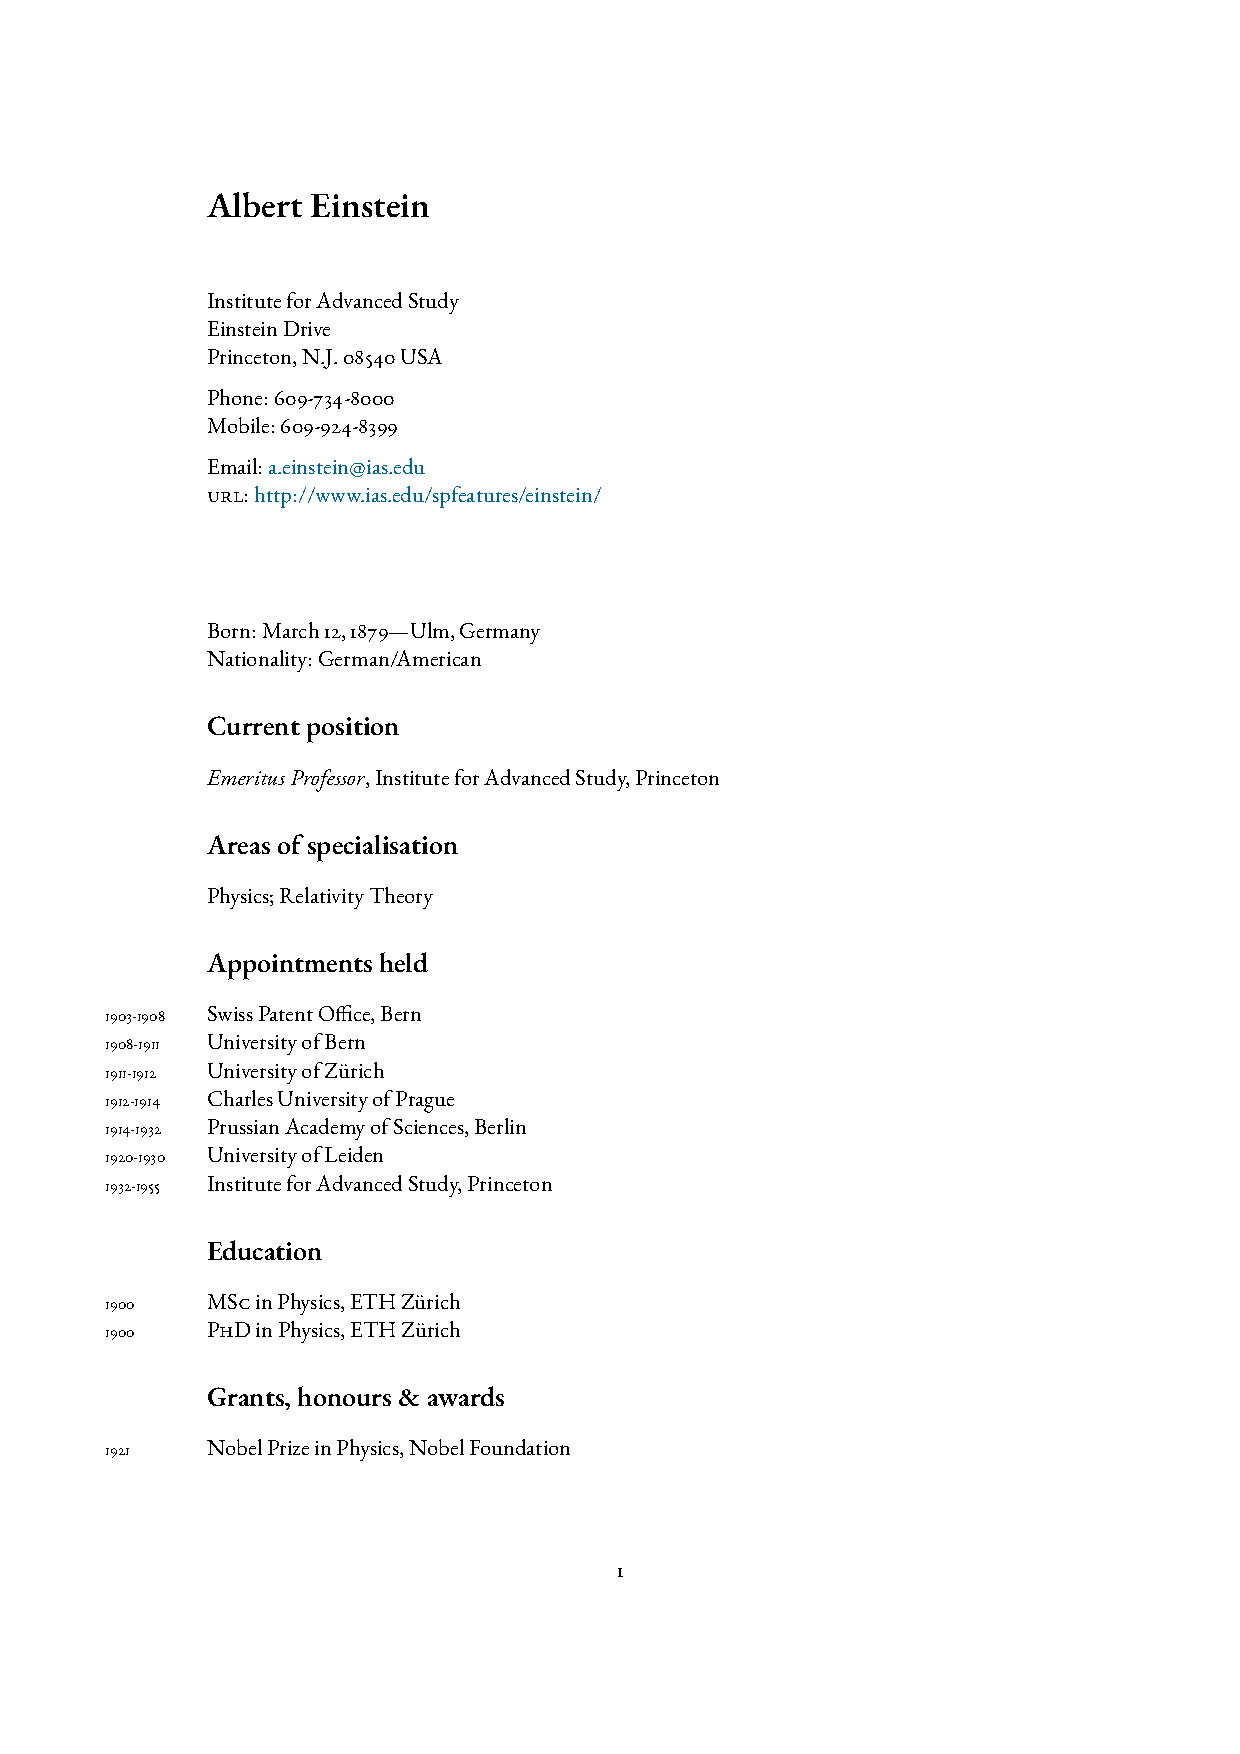
\includepdf[pages=-,pagecommand={},width=1.25\textwidth]{CVs/einstein_cv_latextemplates.pdf}

}

\subsection{J.6 -not required}
\subsection{J.7 - not required in step 1}

\fakesubsection{J.8 MEL}
\iftoggle{subPDFs}{
\begin{landscape}
%\includepdf[pages=1,pagecommand={},angle=90]{MEL.pdf}
\end{landscape}
}

\subsection{J.9 Heritage}

\newpage
%\section{References}

\newpage
\subsection{J.10 List of Abbreviations and Acronyms}

\printglossary[type=main,nonumberlist]
 %to fill this in, run $ makeglossaries main.glo from command line and then compile again.
 
\subsection{J.11 List of References}
\sloppy % keep things from spilling into margins
\bibliographystyle{abbrvnat}
\bibliography{exoplanets}
\end{document}
